\section*{Überblick}

\begin{figure}[htb]
\begin{center}
%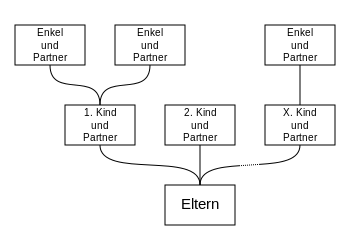
\includegraphics[width=.7\textwidth]{../fig/stammbaum.png}
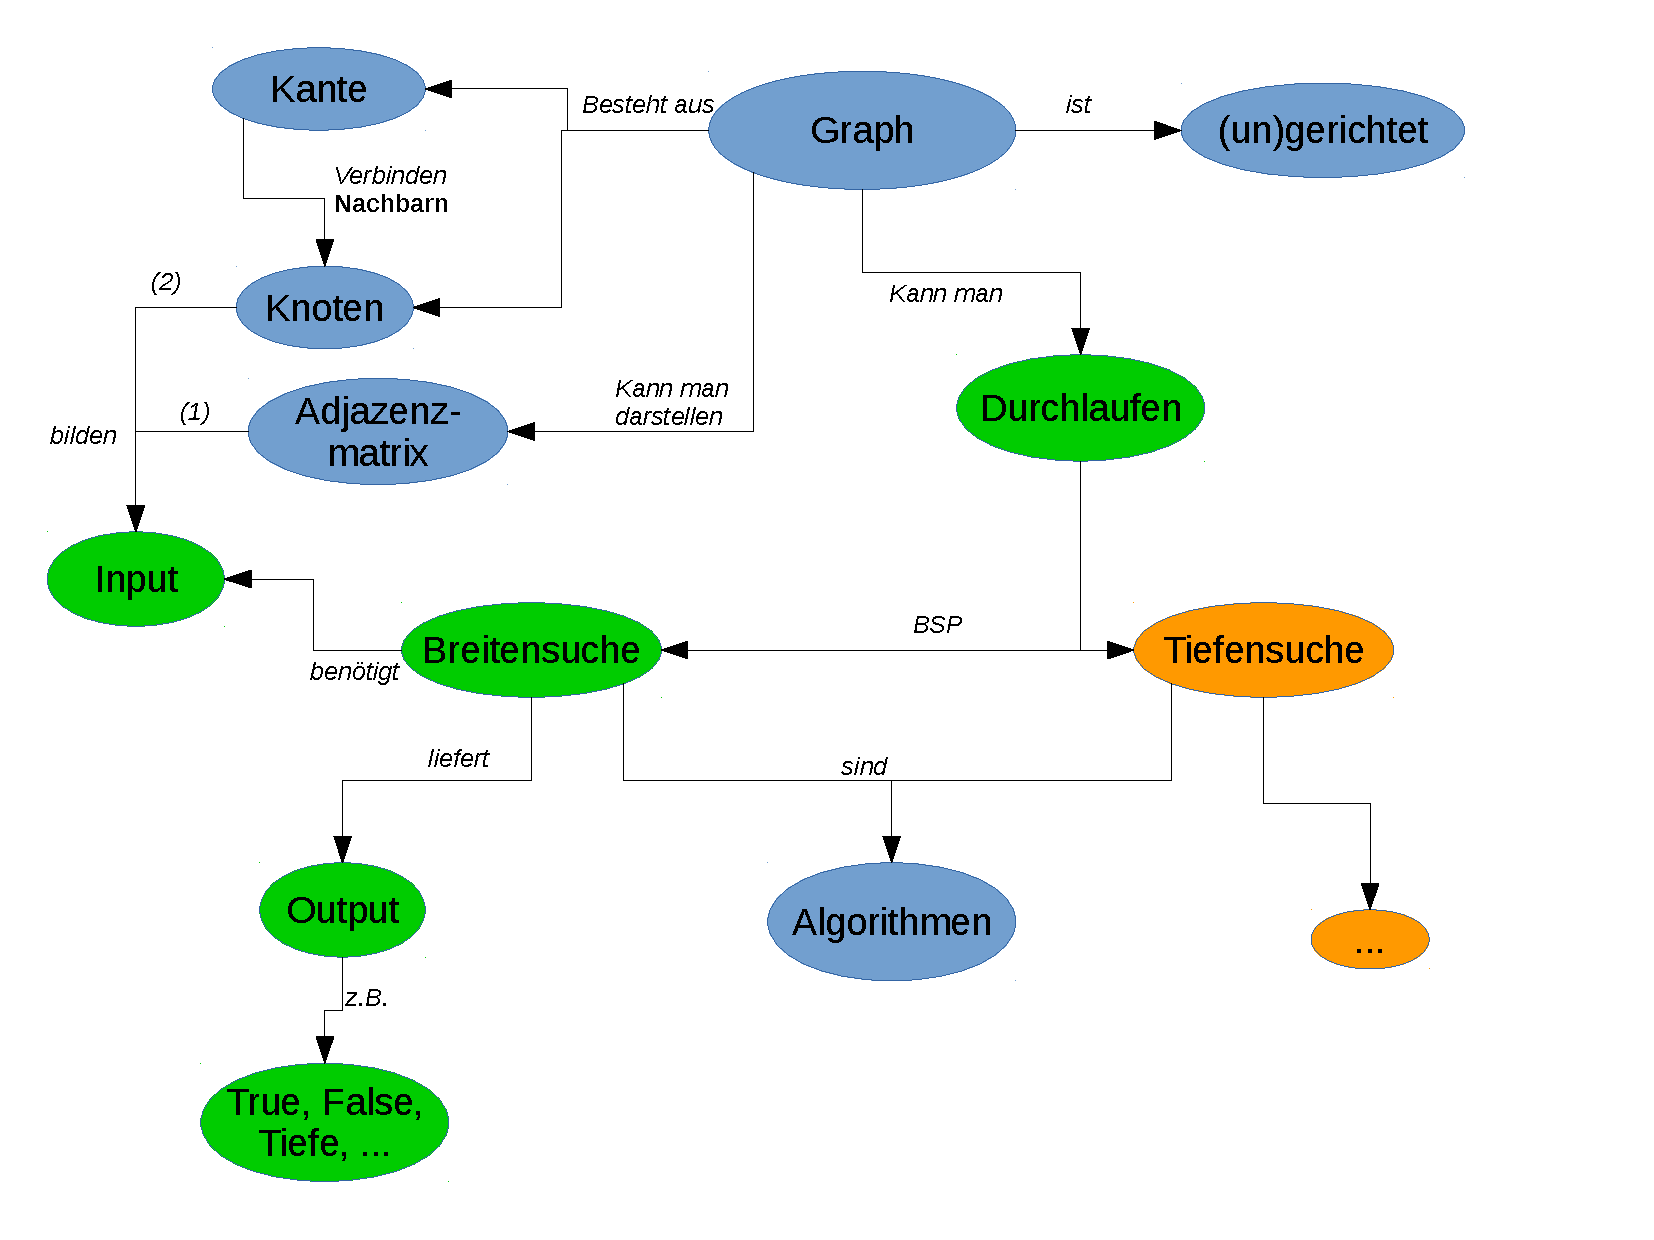
\includegraphics[width=.99\textwidth]{../cmap/bsuche_cmap.pdf}
\caption{Concept-Map zum Thema Breitensuche.
Blaue Konzepte bilden das Vorwissen ab. 
Grüne Konzepte werden in dieser Arbeit eingeführt und behandelt. 
Orangene Konzepte bilden einen Ausblick auf Konzepte, welche im Rahmen dieser Arbeit nicht mehr behandelt werden. 
}
\label{fig:cmap2}
\end{center}
\end{figure}


Den Begriff Graph haben Sie schon einmal gehört. Mit einem Graphen kann man verschiedene Objekte mit einander verbinden. 
Eine interessante Frage ist immer über wie viele Verbindung zwei Objekte mit einander verknüpft sind. 
Wir möchten nun mit diesem Kapitel überlegen, wie man einen Graphen durchsuchen kann.
Ein Beispiel für einen solchen Algorithmus ist die Breitensuche. 
Ziel ist es, dass Sie den Algorithmus verstehen und anwenden können. 

Der Aufbau dieses Kapitels ist so gehalten, dass Sie im ersten Abschnitt nochmal die Grundlagen zu Graphen wiederholen und festigen. 
Dabei geht es vor allem um verschiedene Darstellungen von Graphen und das Konzept von Nachbarn.
Im zweiten Abschnitt sollen dann Grundlagen des Modellierens von Problemen mit Hilfe von Graphen und das L\"osen der Probleme mit Hilfe von Algorithmen auf Graphen vermittelt werden.
Insbesondere werden Problemstellungen betrachtet, die sich mit Hilfe von der eines neuen Algorithmus (\emph{Breitensuche}, lösen lassen. 
Der Algorithmus für die Breitensuche wird dabei Schritt f\"ur Schritt erarbeitet, erweitert und implementiert.

In der Concept-Map (s. Abb.~\ref{fig:cmap2}) können Sie die verschiedenen Konzepte und ihren Zusammenhang für das folgende Kapitel überblicken. 
Mit der Farbe Blau markierte Konzepte stellen sollte schon bekannt sein, aber werden nochmal wiederholt.
Grün markiert sind neue Konzepte, die in dieser Einheit behandelt werden und orange sind Konzepte, die einen Ausblick bilden und nicht mehr behandelt werden. 

